% This file was created with tikzplotlib v0.10.1.
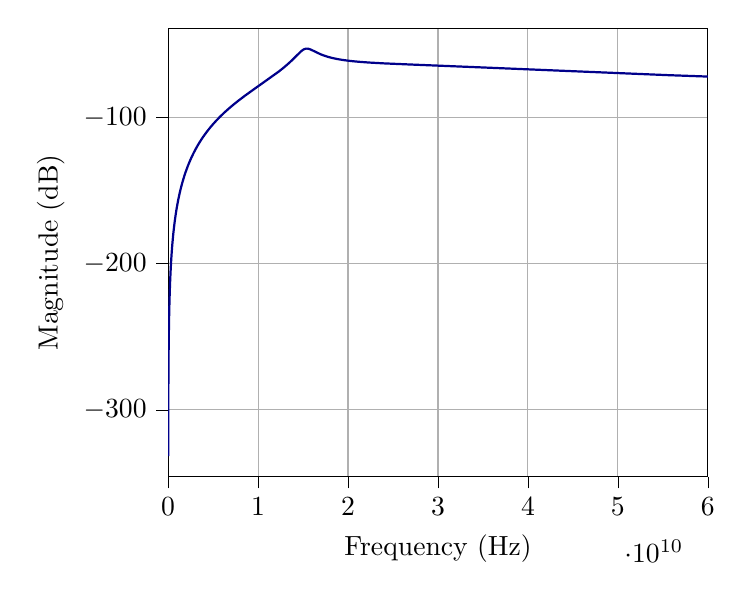
\begin{tikzpicture}

\definecolor{darkblue}{RGB}{0,0,139}
\definecolor{darkgray176}{RGB}{176,176,176}

\begin{axis}[
tick align=outside,
tick pos=left,
x grid style={darkgray176},
xlabel={Frequency (Hz)},
xmajorgrids,
xmin=10000000, xmax=60000000000,
xtick style={color=black},
xtick={0,10000000000,20000000000,30000000000,40000000000,50000000000,60000000000},
%xticklabels={0,10,20,30,40,50,60},
y grid style={darkgray176},
ylabel={Magnitude (dB)},
ymajorgrids,
ymin=-345.545075, ymax=-39.017425,
ytick style={color=black}
]
\addplot [thick, darkblue]
table {%
10000000 -331.611999511719
20000000 -300.544006347656
30000000 -284.372009277344
40000000 -273.535003662109
50000000 -265.368011474609
60000000 -258.802001953125
70000000 -253.302993774414
80000000 -248.570999145508
90000000 -244.414001464844
100000000 -240.707000732422
110000000 -237.360992431641
120000000 -234.311996459961
130000000 -231.509994506836
140000000 -228.919006347656
150000000 -226.509002685547
160000000 -224.255996704102
170000000 -222.141006469727
180000000 -220.147003173828
190000000 -218.261993408203
200000000 -216.475006103516
220000000 -213.154998779297
240000000 -210.125
260000000 -207.339004516602
280000000 -204.759994506836
300000000 -202.360000610352
320000000 -200.115005493164
340000000 -198.00700378418
360000000 -196.018997192383
390000000 -193.235992431641
420000000 -190.658996582031
450000000 -188.261001586914
480000000 -186.018005371094
510000000 -183.910995483398
550000000 -181.285995483398
590000000 -178.84700012207
630000000 -176.567001342773
680000000 -173.912994384766
730000000 -171.447998046875
780000000 -169.147003173828
840000000 -166.572006225586
900000000 -164.175003051758
960000000 -161.932998657227
1030000000 -159.488998413086
1100000000 -157.205001831055
1180000000 -154.766998291016
1270000000 -152.214004516602
1360000000 -149.837005615234
1450000000 -147.611999511719
1550000000 -145.296005249023
1660000000 -142.916000366211
1780000000 -140.49299621582
1900000000 -138.227996826172
2040000000 -135.761001586914
2180000000 -133.457000732422
2329999872 -131.147994995117
2489999872 -128.843002319336
2670000128 -126.420997619629
2860000000 -124.035003662109
3070000128 -121.575996398926
3289999872 -119.172996520996
3540000000 -116.628997802734
3800000000 -114.166000366211
4049999872 -111.948997497559
4339999744 -109.539001464844
4670000128 -106.981002807617
4990000128 -104.661003112793
5369999872 -102.083000183105
5820000256 -99.2404022216797
6270000128 -96.5893020629883
6760000000 -93.8836975097656
7289999872 -91.1322021484375
7880000000 -88.2412033081055
8560000000 -85.0821990966797
9420000256 -81.2705001831055
12250000384 -68.8759994506836
12789999616 -66.2555999755859
13260000256 -63.807201385498
13680000000 -61.4490013122559
14110000128 -58.8574981689453
14739999744 -55.035400390625
14919999488 -54.1342010498047
15070000128 -53.5447998046875
15210000384 -53.1674003601074
15340000256 -52.983699798584
15480000512 -52.9632987976074
15630000128 -53.119800567627
15809999872 -53.4894981384277
16060000256 -54.1916999816895
16940000256 -56.7923011779785
17340000256 -57.7414016723633
17770000384 -58.5905990600586
18269999104 -59.3958015441895
18830000128 -60.1184005737305
19480000512 -60.7811012268066
20259999744 -61.3979988098145
21159999488 -61.9435997009277
22339999744 -62.4847984313965
24060000256 -63.0714988708496
27089999872 -63.8662986755371
35020001280 -65.8541030883789
55630000128 -71.1163024902344
60000002048 -72.0744018554688
};
\end{axis}

\end{tikzpicture}
